\documentclass[a4paper]{report}

%====================== PACKAGES ======================

\usepackage[french]{babel}
\usepackage[utf8x]{inputenc}
%pour gérer les positionnement d'images
\usepackage{float}
\usepackage{amsmath}
\usepackage{graphicx}
\usepackage{amssymb}
\usepackage[colorinlistoftodos]{todonotes}
\usepackage{url}
%pour les informations sur un document compilé en PDF et les liens externes / internes
\usepackage{hyperref}
%pour la mise en page des tableaux
\usepackage{array}
\usepackage{tabularx}
%pour utiliser \floatbarrier
%\usepackage{placeins}
%\usepackage{floatrow}
%espacement entre les lignes
\usepackage{setspace}
%modifier la mise en page de l'abstract
\usepackage{abstract}
%police et mise en page (marges) du document
\usepackage[T1]{fontenc}
\usepackage[top=2cm, bottom=2cm, left=2cm, right=2cm]{geometry}
%Pour les galerie d'images
\usepackage{subfig}
\usepackage{svg}

%====================== INFORMATION ET REGLES ======================

%rajouter les numérotation pour les \paragraphe et \subparagraphe
\setcounter{secnumdepth}{4}
\setcounter{tocdepth}{4}

\setlength{\parskip}{3ex}

\hypersetup{							% Information sur le document
pdfauthor = {Amosse Maxime,
			Hemery Julien,
			Hervieux Hugo,
    		Pascou Sylvain},			% Auteurs
pdftitle = {PinaPL ---
			Projet-long sur les réseaux neuronaux},			% Titre du document
pdfsubject = {Compte rendu de projet},		% Sujet
pdfkeywords = {PinaPL, neuron, \ldots},	% Mots-clefs
pdfstartview={FitH}}					% ajuste la page à la largueur de l'écran
%pdfcreator = {MikTeX},% Logiciel qui a crée le document
%pdfproducer = {}} % Société avec produit le logiciel

%======================== DEBUT DU DOCUMENT ========================

\begin{document}

%régler l'espacement entre les lignes
\newcommand{\HRule}{\rule{\linewidth}{0.5mm}}

%page de garde
% !TeX root = main.tex

\begin{titlepage}
\begin{center}

% Upper part of the page. The '~' is needed because only works if a paragraph
% has started.

\includegraphics[width=0.35\textwidth]{./images/logo.png}~\\[1cm]

\textsc{\LARGE Projet Long - Supélec}\\[1.5cm]

\textsc{\Large }\\[0.5cm]

% titre
\HRule
\\[0.4cm]

{\huge \bfseries PinaPL \\
\mdseries \scriptsize \textit{PinaPL is not a Projet Long} \\
\huge \bfseries Réseaux de neurones \& LSTM \\[0.4cm] }

\HRule
\\[1.5cm]

% Author and supervisor
\begin{minipage}{0.4\textwidth}
\begin{flushleft} \large
\emph{Auteurs:}\\
Maxime \textsc{Amossé}\\
Julien \textsc{Hemery}\\
Hugo \textsc{Hervieux}\\
Sylvain \textsc{Pascou}
\end{flushleft}
\end{minipage}
\begin{minipage}{0.4\textwidth}
\begin{flushright} \large
\emph{Référents:} \\
Arpad \textsc{Rimmel} \\
Joanna \textsc{Tomasik}
\end{flushright}
\end{minipage}

\vfill

% Bottom of the page
{\large \today}

\end{center}
\end{titlepage}


%page blanche
\newpage
%ne pas numéroter cette page
\thispagestyle{empty}
\newpage

% !TeX root = main.tex

\renewcommand{\abstractnamefont}{\normalfont\Large\bfseries}
%\renewcommand{\abstracttextfont}{\normalfont\Huge}

\begin{abstract}
\hskip7mm

%TODO

\begin{spacing}{1.3}

(résumé)

\end{spacing}
\end{abstract}


\renewcommand{\baselinestretch}{0.15}\normalsize
\tableofcontents
\renewcommand{\baselinestretch}{1.00}\normalsize

\thispagestyle{empty}
\setcounter{page}{0}
%ne pas numéroter le sommaire

\newpage

%espacement entre les lignes d'un tableau
\renewcommand{\arraystretch}{1.5}

%====================== INCLUSION DES PARTIES ======================

\thispagestyle{empty}
%recommencer la numérotation des pages à "1"
\setcounter{page}{0}
\newpage

% !TeX root = main.tex

\chapter{Présentation du projet}

\section{Objectifs}

Ce projet a été lancé le 23 septembre 2016 sur proposition de M\textsuperscript{me} Joana \textsc{Tomasik}
et M.\ Arpad \textsc{Rimmel}. Le but est d'implémenter en un peu moins d'un an un algorithme d'apprentissage sur un réseau neuronal avec mémoire appelé LSTM\footnotemark, en étudiant d'autres structures de réseaux plus simples auparavant.

\footnotetext{Long Short Term Memory}

\bigskip

Un tel projet représente de fortes contraintes techniques (implémentation de la structure de
 réseau neuronal, gestion de la mémoire, performances, \ldots) mais aussi un défi
 théorique (élaboration des algorithmes, leur justification formelle, \ldots).

\bigskip

Pour arriver à ce résultat, l'année est découpée en différents grandes étapes et dans
chacune nous devons découvrir et implémenter une spécificité des réseaux
neuronaux.
Tout d'abord nous voulons implémenter un réseau neuronal simple pour
nous familiariser avec le concept des réseaux de neurones et mettre en place
les outils adéquats pour les simuler. Puis, nous modifierons ces réseaux
basiques pour y introduire des propriétés plus complexes, tels les réseaux
récurrents (RTRL, BPTT). Enfin, nous adapterons le réseau et son algorithme pour
qu'il corresponde à celui du LSTM.

\section{Équipe}

L'équipe du projet est composée de quatre élèves-ingénieurs de CentraleSupélec, cursus ingénieur Supélec :
Maxime \textsc{Amossé}, Julien \textsc{Hemery}, Hugo \textsc{Hervieux} et Sylvain \textsc{Pascou}, encadrés par deux
enseignants-chercheurs du même établissement, M\textsuperscript{me} Joana \textsc{Tomasik} et M.\ Arpad
\textsc{Rimmel}.

\section{Outils}

\subsection{Langage de programmation}
Le langage de programmation choisi est le C++, pour sa rapidité d'exécution,
sa grande versatilité, la richesse de sa communauté, ainsi que le aspects pédagogiques de son
utilisation. Il est important de faire remarquer que ce langage est compilé et
donc ne permet donc pas directement à l'utilisateur d'interagir simplement avec les
variables durant l'exécution, ce qui complique significativement les phases de déboggage.

\subsection{Outil de versionnement}

Pour travailler en groupe de manière efficace nous avons utilisé le
gestionnaire de version Git et un dépôt partagé sur la plateforme GitHub :
\url{https://github.com/supelec-lstm/PinaPL}. Il nous a fallu une dizaine
d'heures et quelques règles de bonne conduite pour éviter de créer des
conflits et faciliter le travail de chacun.

\smallskip

Chaque développeur travaille donc sur la branche de la fonction qu'il
implémente, puis il la fusionne dans la branche principale lorsqu'il a une version
stable qui compile et se comporte correctement.

\subsection{Gestion de la bibliographie et références}

Zotero est un outil gratuit de gestion de bibliographie. Il permet à tous les
membres du projet d'y enregistrer des références utiles, des articles papiers,
mais aussi les fichiers PDF contenant lesdits articles.
De plus, il nous permet d'exporter régulièrement la bibliographie sous un
format standard pour l'inclure dans ce rapport.

\subsection{Écriture du présent rapport}

Enfin, pour rédiger ce rapport, nous avons utilisé \LaTeX\xspace. Il s'agit d'un
langage de création de documents axé autour du document
scientifique ; il est reconnu par la communauté pour sa facilité d'utilisation
et sa capacité à générer des documents propres et ordonnés.

% !TeX root = main.tex

\chapter{Réseau neuronal simple}

\section{Théorie}

\subsection{Le perceptron}

Le perceptron est le neurone le plus basique que l'on puisse trouver dans la
littérature. Un perceptron est défini par :
\begin{itemize}
\item $n$ entrées $x_i$
\item $1$ sortie $y$
\item $n$ poids $w_i$
\item $1$ biais $\theta$
\item $1$ fonction de composition $g : \mathbb{R}^n \to \mathbb{R}$
\item $1$ fonction d'activation $f : \mathbb{R} \to \mathbb{R}$
\end{itemize}

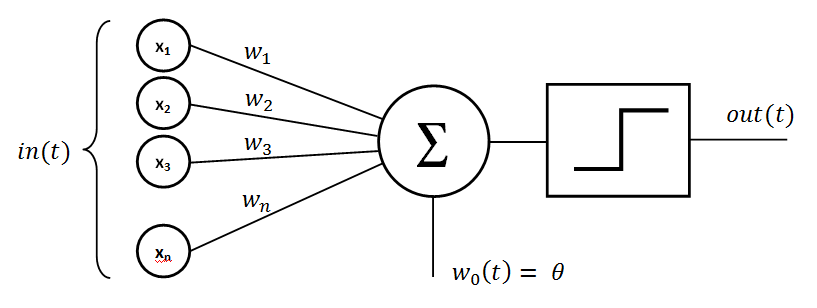
\includegraphics[scale=0.8]{images/perceptron.png}

\vspace{\parskip}
Sur sa construction, le perceptron est fortement inspiré sur le neurone humain,
sans pour autant en être une représentation réaliste.
Le perceptron détermine avec ses entrées si il "active" ou non la sortie, c'est
à dire s'il relaie le signal. Pour cela il rassemble toutes les données des
entrées $x_i$ à l'aide de la fonction de composition $g$. Le neurone ne donnant
pas la même importance à chaque entrée, on les pondère préalablement par les
poids notés $w_i$.
Finalement, on décide du signal de sortie à l'aide de la fonction d'activation
$f$. De base, le seuil d'activation est souvent centré en $0$. Pour palier à ce
problème, on prend également en entrée de la fonction d'activation un biais
$\theta$.

\medskip

En résumé, on a :
\[y = f(g(x_1w_1, x_2w_2, \ldots , x_nw_n) + \theta) \]

\medskip

Usuellement, la fonction d'activation est la somme :
\[y = f(\sum_{i=1}^n x_iw_i + \theta) \]

\medskip

On remarque que le biais agit comme le poids d'une entrée du neurone qui serait
toujours $1$.

\subsection{Le réseau}

Une réseau de neurones permet de créer des fonctions de bien plus grande
complexité qu'un simple neurone, permettant de résoudre des problèmes
jusqu'alors inaccessibles à la machine. Il permet par exemple de faire des
classifications sur le MNIST. Le MNIST est un problème classique où l'on a des
images resprésentant des chiffres manuscrits et pour lequel l'on doit déterminer
 le chiffre représenté. C'est un problème d'une extrême simplicité pour un être
 humain, mais presque impossible à résoudre avec une programmation classique
sans réseau neuronal. Ainsi, pour construire un réseau, chaque perceptron est
mis en relation avec ses pairs (un perceptron prend en entrée les sorties
d'autres perceptrons). On construit alors un graphe orienté dans lequel chaque
sommet est un perceptron. On se limitera dans un premier temps au cas d'un
réseau acyclique.

\bigskip

On peut définir plusieurs types de neurones dans un réseau :
\begin{itemize}
\item les neurones d'entrée
\item les neurones cachés
\item les neurones de sortie
\end{itemize}

\bigskip

Il faut donc autant de neurones d'entrée que de dimensions qu'a l'échantillon
que l'on veut soumettre au réseau. Par exemple dans le cadre du MNIST (insert cite here)
on veut en entrée une image de dimension $28 \times 28$, on place donc $784$
neurones d'entrées. En pratique, les neurones d'entrée sont des neurones fictifs
; ils sont présents pour faciliter la construction du réseau de neurone.
En effet, ils ne sont soumis à aucun apprentissage et leur sortie est la même
que leur entrée. Nous ne les considérerons pas dans la théorie qui suit.

\medskip

Les neurones des couches cachées sont présents entre les neurones d'entrée et de
 sortie. Ils sont utiles uniquement pour le calcul de la sortie. Le nombre de
 couches et la taille des couches influent sur l'action du réseau. Un réseau à
 multiples couches cachées sera capable de traiter des problèmes beaucoup plus
 complexes qu'un réseau à simple couche cachée. Il est évident que cela augmente
  néanmoins la complexité des calculs et le temps d'exécution.

\medskip

Les neurones de sortie sont ceux qui servent pour la classification de
l'échantillon d'entrée. Si l'on souhaite classifier une entrée il faut le même
nombre de neurones de sortie que de classes différentes possibles. Ainsi dans
l'exemple du MNIST, le but est de déterminer un chiffre donné sur une image.
Il y a donc $10$ possibilités (les 10 chiffres). Il y a donc $10$ neurones de
sortie.

\medskip

Par la suite, on appellera $\{x_i\}_{i \leq n}$ les entrées, $\{y_i\}_{i \leq m}$
 les sorties des neurones $\{y_i\}_{m+1-M \leq i \leq m}$ les sorties des
neurones de sorties, $\{\sigma_i\}_{i \leq m}$ les fonctions d'activations et
$\{\theta_i\}_{i \leq m}$ les biais.

\medskip

On définit enfin $\{F_i\}_{i \leq m}$ tel que $j \in E_i$ si et seulement si la
sortie du neurone $j$ est reliée au neurone $i$. On peut ainsi numéroter les
poids : $\{w_{ij}\}_{i \leq m, j \in F_i} $ le poids associé à l'entrée reliant
le neurone $j$ au neurone $i$.

\medskip

D'après ce qui précède, on obtient $\forall i \in [1, m]$ :

\[y_i = \sigma_i(\sum_{j \in F_i} y_jw_{ij} + \theta_i) \]

\subsection{Les réseaux à couche}

Il existe un type de réseau simplifié très utilisé. On partitionne l'ensemble
des neurones en $K$ ensembles. On chacun de ces ensembles une "couche". De plus,
chaque neurone d'une couche a comme entrées l'ensemble (ou partie) des sorties
des neurones de la couche précédente. On notera $\alpha^{(k)}_j$ l'élément $j$
de la couche $k$ de $\alpha$. On notera également $N_k$ le nombre de neuroneq à
la couhce $k$. On a donc pour tout $k > 1$ :

\[y_i^{(k)} = \sigma_i^{(k)}(\sum_{j = 0}^{N_{k-1}} y_j^{(k-1)}w_{ij}^{(k)} + \theta_i^{(k)}) \]

On remarque que l'on peut simplifier la notation en considérant la formule
ci-dessus avec une approche vectorielle :

\[\overline{y^{(k)}} = w^{(k)} \times y^{(k-1)} + \theta^{(k)}\]
\[y^{(k)} = \sigma^{(k)}(\overline{y^{(k)}}) \]

On peut montrer que tout réseau acyclique peut se ramener à un réseau à couches
dont certains poids sont imposés comme nuls. Nous prenons donc l'hypothèse que
le réseau est un réseau à $K$ couches, que la première couche est l'ensemble des
 neurones d'entrée et la dernière couche l'ensemble des neurones de sortie, sans
 perte de généralité.

\subsection{L'apprentissage}

L'efficacité d'un réseau de neurones se mesure à la qualité de sa classification
. Celle-ci dépend des poids qui sont attribués à chacune de ses entrées. Il faut
 donc déterminer la bonne combinaison de poids qui permettra au réseau de
simuler la fonction voulue. Le nombre de poids présents dans un réseau augmente
très rapidement et il devient complexe d'estimer cette bonne combinaison. Pour
cela, on procède à une phase apprentissage : on utilise un échantillon de
données dont on connaît le résultat pour construire un réseau avec les bon poids
. On part ainsi d'un réseau avec des poids aléatoires, choisis dans un
intervalle restreint et centré en zéro, et on les modifie en prenant en compte
les erreurs entre les valeurs obtenues et les valeurs théoriques. Dans la suite,
 on s'intéressera à toute la démarche nécessaire pour arriver à cette modification de poids.

\medskip

On notera $\{x_i\}_{i \leq n}$ et $\{Y_i\}_{i \leq M}$ les entrées et sorties
des échantillons.

\medskip

Pour déterminer les modifications à effectuer, on calcule la sortie du réseau de
 neurones à un échantillon de test donné et on mesure l'erreur. Pour cela,
on choisira une fonction qui mesurera la différence entre le vecteur de sortie
et le vecteur des sorties théoriques. Classiquement, on utilise la méthode des
moindres carrés $E_m$ ou bien une fonction softmax à laquelle on rajoute une
entropie croisée $E_s$:

\[E_m = \sum_{j = 1}^{M} \cfrac{(Y_j - y_j^{(K)})^2}{2}\]
\[E_s = \sum_{j = 1}^{M} Y_j \log \left(\cfrac{e^{y_j^{(K)}}}{\sum e^{y_i^{(K)}}}\right)\]

\subsection{La méthode des gradients}

On veut donc minimiser $E$ en modifiant les $w_{ij}$. Le problème ici est que
l'on a une connaissance limitée de $E$ en fonction des $w_{ij}$ car on ne
dispose des valeurs théoriques de sortie que pour un nombre fini de valeurs. Or
les méthodes de minimisation de fonctions reposent souvent sur une connaissance
continue de ce que l'on veut optimiser. La seule méthode viable est la méthode
des gradients.

\medskip

On a une fonction $f$, appelée fonction de coût, que l'on veut minimiser par
rapport à un facteur $x$. On crée alors une suite $(x_n)$ telle que
$x_{n+1} = x_{n} - \cfrac{\partial f}{\partial x}(x_n)$.
L'idée est se déplacer sur le potentiel de $f$ grâce à son gradient. Avec cette
méthode, on peut calculer facilement la suite $(x_n)$ car il suffit d'évaluer
le gradient en un point et non plus en un nombre continuement infini.

\medskip

Cependant, cette méthode est imprécise et il arrive qu'elle converge vers un
minimum local. En pratique, l'ajout de neurones va augmenter le nombre de
dimensions du gradient et donc permettre de limiter le nombre de minima locaux.

\medskip

\subsection{La rétropropagation}

D'après ce qui précède, l'objectif est donc d'évaluer pour tout $w_{ij}^{(k)}$ :
 $\cfrac{\partial E}{\partial w_{ij}^{(k)}}$.

\begin{align*}
\cfrac{\partial E}{\partial w_{ij}^{(k)}} &= \sum_{l = 1}^{M} \cfrac{\partial y_l^{(K)}}{\partial w_{ij}^{(k)}} \times \cfrac{\partial E}{\partial y_l}\\
&= \left\langle\cfrac{\partial y^{(K)}}{\partial w_{ij}^{(k)}},\cfrac{\partial E}{\partial y}\right\rangle\\
&= \left\langle\cfrac{\partial \overline{y^{(K)}}}{\partial w_{ij}^{(k)}} \odot \sigma'(\overline{y}),\cfrac{\partial E}{\partial y}\right\rangle \\
&= \left\langle\cfrac{\partial \overline{y^{(K)}}}{\partial w_{ij}^{(k)}} ,\sigma'(\overline{y^{(K)}}) \odot \cfrac{\partial E}{\partial y}\right\rangle
\end{align*}

Calculons maintenant $\cfrac{\partial \overline{y^{(l)}}}{\partial w_{ij}^{(k)}}$.
Tout d'abord, remarquons que si $l = k$ alors on a simplement :

\[\cfrac{\partial \overline{y^{(k)}}}{\partial w_{ij}^{(k)}} = E_{ij} y^{(k-1)} = y^{(k-1)}_j e_i\]

Ceci vient du fait que le réseau étant acyclique, $ y^{(l)}$ ne dépend pas de
$w_{ij}^{(k)}$ pour $l < k$. De même, pour $l > k$, on obtient :

\begin{align*}
\cfrac{\partial \overline{y^{(l)}}}{\partial w_{ij}^{(k)}} &= w^{(l)} \times \cfrac{\partial y^{(l-1)}}{\partial w_{ij}^{(k)}}\\
&= w^{(l)} \times \left(\sigma(\overline{y^{(l-1)}}) \odot \cfrac{\partial \overline{y^{(l-1)}}}{\partial w_{ij}^{(k)}}\right)
\end{align*}

Donc en supposant qu'il existe un vecteur $v$ tel que $\cfrac{\partial E}{\partial w_{ij}^{(k)}} = \left\langle\cfrac{\partial \overline{y^{(l)}}}{\partial w_{ij}^{(k)}} ,v\right\rangle$ :

\begin{align*}
\cfrac{\partial E}{\partial w_{ij}^{(k)}} &= \left\langle w^{(l)} \times \left(\sigma(\overline{y^{(l-1)}}) \odot \cfrac{\partial \overline{y^{(l-1)}}}{\partial w_{ij}^{(k)}}\right) ,v\right\rangle\\
&= \left\langle\sigma(\overline{y^{(l-1)}}) \odot \cfrac{\partial \overline{y^{(l-1)}}}{\partial w_{ij}^{(k)}},{}^t \! w^{(l)} \times v\right\rangle\\
&= \left\langle\cfrac{\partial \overline{y^{(l-1)}}}{\partial w_{ij}^{(k)}},\sigma(\overline{y^{(l-1)}}) \odot ({}^t \! w^{(l)} \times v)\right\rangle\\
\end{align*}

Donc il existe $u = \sigma(\overline{y^{(l-1)}}) \odot ({}^t \! w^{(l)} \times v)$
tel que $\cfrac{\partial E}{\partial w_{ij}^{(k)}} = \left\langle\cfrac{\partial \overline{y^{(l-1)}}}{\partial w_{ij}^{(k)}} ,u\right\rangle$

Donc par récurrence, pour tout $l \geq k$ il existe $\delta y^{(l)}$ tel que :
\[\cfrac{\partial E}{\partial w_{ij}^{(k)}} = \left\langle\cfrac{\partial \overline{y^{(l)}}}{\partial w_{ij}^{(k)}} ,\delta y^{(l)}\right\rangle\]

On remarquera que $\delta y^{(l)}$ ne dépend pas de $w_{ij}^{(k)}$. On appellera
 $\delta y^{(l)}_j$ le gradient du neurone $j$ de la couche $l$. Ce gradient vérifie la relation de reccurence suivante d'après ce qui précède :

\[
\left \{
\begin{array}{c @{=} c}
    \delta y^{(K)} & \sigma'(\overline{y^{(K)}}) \odot \cfrac{\partial E}{\partial y}\\
    \delta y^{(k)} & \sigma(\overline{y^{(k)}}) \odot ({}^t \! w^{(k+1)} \times \delta y^{(k+1)})\\
\end{array}
\right.
\]

On a alors :

\begin{align*}
\cfrac{\partial E}{\partial w_{ij}^{(k)}} &= \left\langle\cfrac{\partial \overline{y^{(k)}}}{\partial w_{ij}^{(k)}} ,\delta y^{(k)}\right\rangle\\
&= \left\langle y^{(k-1)}_j e_i,\delta y^{(k)}\right\rangle\\
& = y^{(k-1)}_j \times \delta y^{(k)}_i
\end{align*}

Donc :

\[\Delta w^{(k)}_{ij} = \lambda \times y^{(k-1)}_j \times \delta y^{(k)}_i\]

\[\Delta w^{(k)} = \lambda \times (\delta y^{(k)} \times {}^t \! y^{(k-1)})\]

On obtient donc un algorithme d'apprentissage qui se fait en deux temps : tout
d'abord le calcul du gradient qui se fait récursivement, puis le calcul de la
différence de poids à appliquer. On remarque dans ce cas que l'on propage le
gradient de la fin du réseau vers le début. C'est ceci qui donne le nom à la
méthode employée : la rétropropagation.

\section{L'implémentation}

\subsection{Le neurone}

Le neurone est une classe, il a pour attributs :
\begin{itemize}
  \item le nombre de ses entrées (\verb+int+).
  \item les valeurs de ses entrées (\verb+vector<double>+).
  \item les poids qu'il leur attribue (\verb+vector<double>+).
  \item son biais (\verb+int+).
  \item sa fonction de composition (\verb+compositionFunction+).
  \item sa fonction d'activation (\verb+activationFunction+).
\end{itemize}

\medskip

Il dispose des méthodes suivantes :
\begin{itemize}
  \item \verb+description()+ : indique l'état du neurone.
  \item \verb+reset()+ : remet à zero ses entrées et sa sortie.
  \item les getters et les setters pour les poids, le nombre d'entrées, les
  fonctions de composition...
  \item \verb+calculateOutput()+ : calcul la sortie du neurone en fonction
  de ses entrées.
  \item \verb+getActivationDerivative+ : calcul de la dérivée de la fonction
  d'activation au point observé.
  \item \verb+getCompositionDerivative+ : idem pour la fonction de composition.
\end{itemize}

\subsection{Le réseau}

Le réseau est aussi implémenté en tant que classe.
Un réseau dispose :
\begin{itemize}
  \item d'un nom (\verb+string+).
  \item d'une date de création (\verb+string+).
  \item de ses neurones (\verb+vector<Neuron>+).
  \item de la liste de ses neurones d'entrée (\verb+vector<unsigned long>+).
  \item de la liste de ses neurones de sortie (\verb+vector<unsigned long>+).
  \item de la matrice des liens entre neurones (\verb+vector<vector<double>>+).
  \item de son facteur d'apprentissage (\verb+unsigned long+).
  \item de ses valeurs en entrée (\verb+vector<double>+).
  \item de la matrice des sorties des neurones (\verb+vector<double>+).
\end{itemize}

\medskip

Il dispose des méthodes nécessaires à la propagation du signal ainsi qu'à
sa rétropropagation.

\subsection{Améliorations apportées}

Nous avons ensuite amélioré le code pour diminuer le temps de calcul et clarfier
la structure. Les éléments à améliorer sont :
\begin{itemize}
\item La structure orientée objet
\item Le single-threading
\item calcul à chaque pas des sorties de chaque neurone
\end{itemize}

\medskip

Nous nous sommes progressivement débarrassés de la structure d'objet du neurone
en effectuant les conversions suivantes :

\medskip

\begin{tabular}{c|c}
   structure objet & nouvelle structure \\
   \hline
   neurones.poids + matrice des poids + matrice des relations & matrice des poids \\
   neuron.activationFunction & vecteur de fonctions d'activation \\
   neuron.compositionFunction & on ne considère plus que la somme \\
   neuron.inputs/output & vecteur des entrées/sorties de tout le réseau \\
   neuron.bias & vecteur des biais de chaque neurone du réseau \\
   dérivée de la fonction de composition & vaut 1
\end{tabular}

\medskip

De plus, nous avons déterminé en amont les neurones voisins qui nécessitaient
un rafraîchissement de leur sortie. Cela permet de ne pas calculer à chaque
itération la sortie de tous les neurones du réseau. Lors de la création du
réseau est construite une liste de vecteurs des neurones dont il faut évaluer
la sortie au tour $i$.

\section{Résultats}

Après une longue période de débogage, nous avons obtenu des résultats
satisfaisants.

TODO

\subsection{Le XOR}

TODO

\subsection{Le MNIST}

Les données du problème du MNIST sont réparties en deux fichiers :
\begin{itemize}
    \item Le set d'apprentissage qui contient 60000 entrées (images de 784 pixels
          des chiffres manuscrits suivis des données des chiffres représentés)
    \item Le set de test qui contient 10000 entrées (différentes de celle du set
          d'apprentissage)
\end{itemize}

\medskip

Les valeurs des entrées sont stockées dans les fichiers entre 0 et 255, nous
les avons centrées et normalisées (entre $-0.5$ et $0.5$).

\medskip

Tous les résultats présentés par la suite sont établis en soumettant au réseau
après apprentissage les 10000 entrées du set de test et en comparant la sortie
attendue et la sortie obtenue. On obtient le résultat du calcul du réseau en
prenant la sortie du réseau avec la valeur maximale.

\subsubsection{Le classificateur linéaire}

En créant un réseau neuronal sans bias ni couche cachées on obtient un
classificateur linéaire. Les 10 neurones de sortie sont reliés chacun aux 784
neurones d'entrées. Les poids sont initialisés aléatoirement entre -1 et 1 selon
 une loi uniforme. La fonction d'activation est une siogmoïde, la composition
est une somme pondérée, et la fonction de coût est l'écart quadratique. Le
facteur d'apprentissage $\lambda$ est fixé à $0.3$ en accord avec la littérature
 sur le sujet.


\medskip

Les résultats d'un tel réseau sont forts intéressants car permettent après un
apprentissage stochastique des 60000 échantillons de test d'obtenir un
pourcentage moyen d'erreur de XX \%. (Moyenne effectuée sur 100 réalisations).

TODO

\subsubsection{Réseau sans couche cachées}

\subsection{Réseau avec 1 couche cachée}

\subsubsection{Réseau avec deux couches cachées}

% !TeX root = ../main.tex

\chapter{Real time reccurent learning}

A partir de cette section, les objectifs sont de reconnaître une chaine de caractère en temps réel : c'est à dire que en donnant un ou plusieurs caractères , on doit être capable de prédire la fin de la chaine.
Ce genre de problème peut être étendu à la recherche comportementale en temps réel.
Pour résoudre ce genre de problème, on utilise des réseaux neuronaux récurrents, qui ont l'avantage de se souvenir des états précédents pour pouvoir prédire efficacement les états suivants; ils comportent une mémoire courte.
Dans un premier temps, nous allons nous intéresser aux réseaux RTRL.

\section{Théorie}

Dans la suite, nous allons nous intéresser au problème de la grammaire de Reber, qui servira d'échantillon de test pour RTRL.

\subsection{La grammaire de Reber}

Une grammaire de Reber est un langage défini par l'automate déterministe cyclique suivant :

\begin{figure}[!ht]
\begin{center}
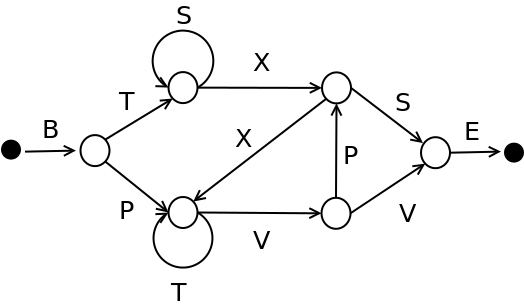
\includegraphics[scale=0.4]{images/reberGrammar.png}
\end{center}
\caption{Grammaire de Reber simple}
\end{figure}


De base, on considère une probabilité uniforme de choisir l'état suivant parmi les états possibles suivants.
La lettre $B$ et la lettre $E$ sont des lettres indiquant simplement le début et la fin de la chaîne, elles n'ont pas d'intérêt propre pour la grammaire.
Les autres lettres présentes sur les arêtes peuvent variées, mais elles doivent respecter les règles suivantes :
\medskip
\begin{itemize}
	\item Chaque lettre doit apparaitre exactement deux fois
	\item On ne peut pas obtenir deux lettres consécutives en passant par des états différents.
\end{itemize}
\vspace{\parskip}
L'intérêt de la grammaire de Reber est que c'est un automate simple qui ne nécessite que la mémoire de la dernière et de l'avant dernière lettre pour trouver la suivante.
En effet, d'après la dernière règle, connaitre les deux dernières lettres impose l'état actuel dans l'automate.
En outre, chaque lettre apparaissant deux fois, la connaissance seule de la dernière lettre ne suffit pas à prédire la suivante correctement.
On remarque que l'on peut résoudre ce problème avec un perceptron classique si on donne en entrée du perceptron les deux dernières lettres du mot.
Ce modèle bien que résolvant ce problème, n'est pas adapté au calcul en temps réel.
De plus il ne résout pas le problème de la grammaire de Reber double.

Le problème de la grammaire double est un problème similaire à la grammaire
simple. L'automate le représentant est :

\begin{figure}[!ht]
\begin{center}
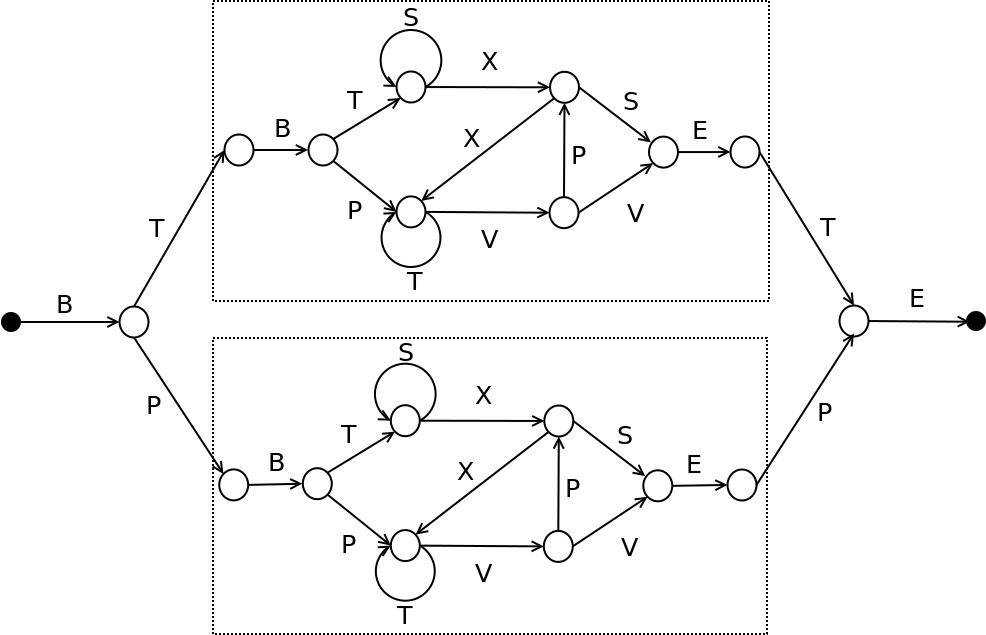
\includegraphics[scale=0.4]{images/reberGrammarSymmetric.png}
\end{center}
\caption{Grammaire de Reber symétrique}
\end{figure}

On remarque qu'il est constitué de deux grammaires de Reber simple qui sont reliés en entrée et en sortie.
La difficulté de ce problème est qu'il faut mémorisé la première valeur pour en déduire la dernière.
Dans ce cas, une mémoire ''infini'' est nécessaire théoriquement pour se souvenir de la première entrée.
Il est donc impensable d'utiliser de la même façon un réseau de perceptron classique. On a alors besoin de réseau récurrent, dont la sortie à un instant $t$ va dépendre de la sortie à un instant $t-1$.

\subsection{Réseau RTRL}

Le principe d'un réseau récurrent est d'utiliser le résultat obtenue par la sortie précédente à l'entrée du calcul suivant.
On aura donc en appelant $x(t)$ la donnée en entrée à l'instant $t$ et $y(t)$ la sortie associé.
On a alors $y(t) = f(x(t), y(t-1))$.
En appelant $\alpha$ un paramètre de la fonction $f$.
Le but est de faire un apprentissage sur $\alpha$ pour minimiser à chaque temps $t$ l'erreur $E(t)$ entre la sortie théorique et la sortie pratique.
De la même façon que précédemment, on va donc calculer $\cfrac{\partial E(t)}{\partial \alpha}$ pour utiliser la méthode du gradient :
Dans un premier temps, nous allons nous intéresser au cas où $f$ est de la forme :

\[ f(x(t), y(t-1)) = \sigma\left (W x(t) + R y(t-1) + b\right )\]

Avec $W$, $R$ qui sont des matrices de poids, $b$ un biais et $\sigma$ une fonction d'activation.
On reconnait donc d'après ce qui précède la formule d'un réseau perceptron à $0$ couche caché et "fully connected".
On pose $\overline{y(t)} = W\times x(t) + R\times y(t-1) + b$.
Les paramètres du systèmes sont donc les éléments de la matrice
On obtient donc pour l'apprentissage :

\[\cfrac{\partial E(t)}{\partial \alpha} = \left\langle \cfrac{\partial y(t)}{\partial \alpha}, J_E \right\rangle\]

\begin{figure}[!ht]
\begin{center}
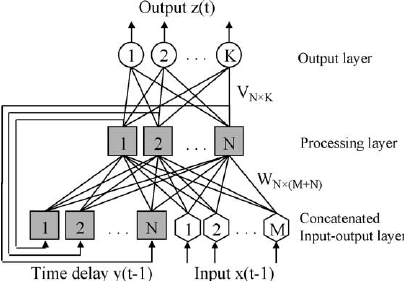
\includegraphics[scale=0.8]{images/rtrl.png}
\end{center}
\caption{Réseau récurrent RTRL}
\end{figure}

\section{Implémentation}

\section{Résultats}
\subsection{Grammaire de Reber simple}
\subsection{Grammaire de Reber double}

% !TeX root = main.tex

\chapter{Back Propagation Through Time}
L'algorithme BPTT appliqué à un réseau neuronal récurrent a pour particularité
de déplier le temps dans l'espace; par exemple, pour apprendre un mot de cinq
caractères, on va créer cinq réseaux non-récurrents qui représentent chaqun un
"temps", soit une lettre de la séquence.

\medskip

Cet algorithme a pour avantage, par rapport à celui RTRL, d'avoir une
complexité temporelle inférieure.

\section{Théorie}

\begin{figure}[!ht]
\begin{center}
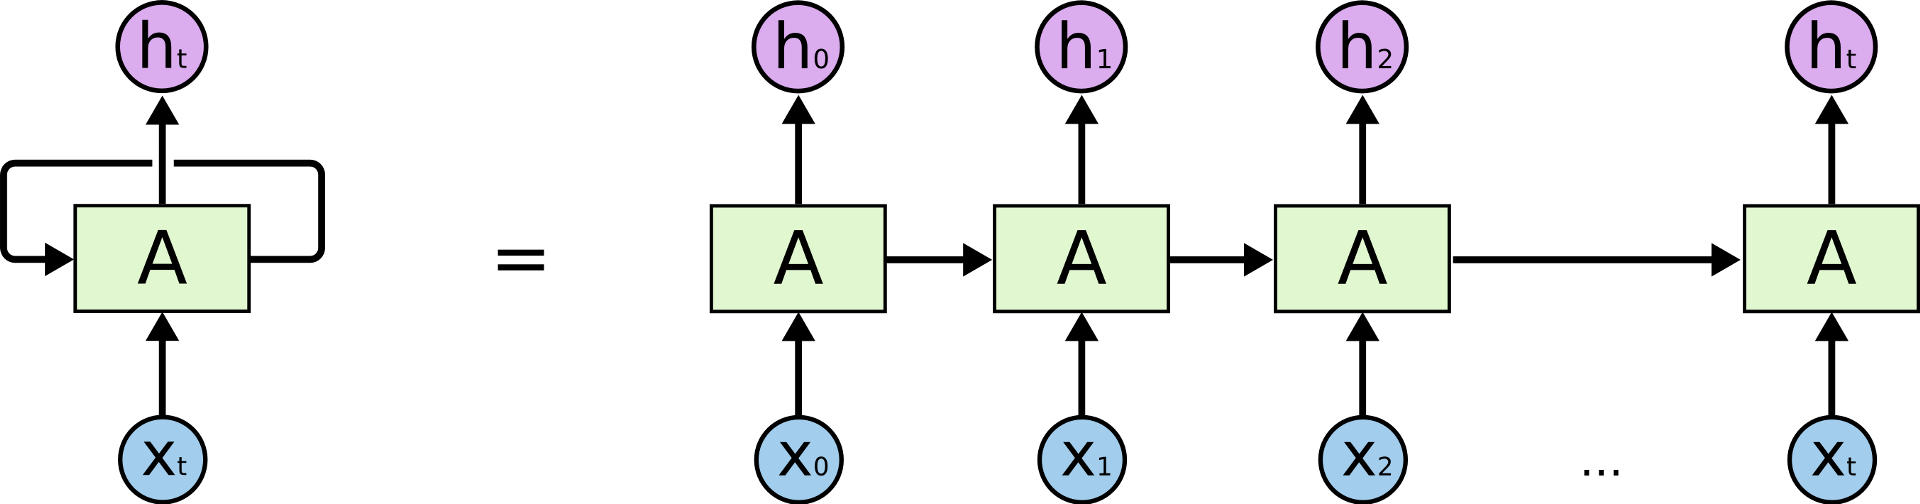
\includegraphics[width=0.8\textwidth]{images/bptt.png}
\caption{Dépliement du temps dans l'espace pour BPTT}
% TODO : crédits
\end{center}
\end{figure}


\subsection{Réseau BPTT}

\section{Implémentation}

L'implémenation est effectuée en C++ via la librairie de calcul matriciel
Eigen3. Toutes les matrices sont des objets de type Eigen::MatrixXd (matrice de
double) et les vecteurs des objets de type Eigen::VectorXd.

\medskip

L'aléatoire utilisé est celui natif en C et C++ : rand.
La génération de la graine se fait à partir du temps à la milliseconde pour
éviter une initialisation déterministe dans le cas de l'execution de plusieurs
runs consécutifs. Pour cela la librairie 'sys/time.h' est utilisée, avec un
appel propre aux systèmes UNIX.

\bigskip

\subsection{Structure de données}

Le code se décompose en plusieurs éléments :
\begin{itemize}
  \item Les poids
  \item Une couche de neurones fully-connected
  \item Le réseau de couches dépliées dans le temps
\end{itemize}

\subsubsection{Les poids}

La classe poids est principalement constituée d'une matrice de poids (carée, de
taille le nombre de neurones). Y est associée une matrice de vartiation de poids
dans laquelle sont stockées toutes les varaitions de poids avant d'être
appliquées. Enfin, il existe un vecteur de biais \verb+bias+ et son vecteur
de variation \verb+delta_bias+ associé.

Enfin, les méthodes de l'objet Poids sont le constructeur et
l'application des variations de poids (qui remet par la même occasion à 0
les delta-poids).

\subsubsection{La couche de neurones}

La couche de neurones (fully-connected) est l'objet élémentaire du réseau. Elle
représente la réseau à un instant t. Elle est crée lors de la propagation d'un
vecteur en entrée à l'instant t et prend en argument un pointeur vers un objet
de type Poids ainsi que ses dimentions.

\medskip

Elle dispose des methodes nécessaires à la propagation et la rétropropagation
d'une entrée à travers le réseau à une couche, stocke ses entrées et sorties
pour les réutiliser lors de la rétropropagation. Lors de la propagation, elle
prend en entrée un vecteur d'entrées et renvoie un vecteur des sorties de
ses neurones. De même, lors de la rétropropagation elle prend en entrée un
vecteur de gradient et en renvoie un autre en sortie. Lors de la
rétropropagation elle calcule aussi les variations de poids à appliquer et les
ajoute au \verb+delta_weight+ de son objet Poids.

\medskip

La fonction d'activation choisie est la sigmoide, la fonction de composition
est la somme, et la fonction de coût est la moitié du coût quadratique (pour
pouvoir dériver plus rapidement).

\medskip

Les attributs de la couche de neurones sont donc les suivants :

\begin{itemize}
  \item \verb+Weights* weights+ l'objet poids qui sera utilisé pour calculer
    les sorties de chaque noeud ;
  \item \verb+Eigen::VectorXd input+ vecteur des entrées de la couche à
    l'instant $t$ ;
  \item \verb+Eigen::VectorXd previous\_output+ vecteur des sorties de la
    couche à l'instant $t-1$ ;
  \item \verb+Eigen::VectorXd output+ sortie de la couche à l'instant $t$.
\end{itemize}

Les méthodes sont donc les suivantes :

\begin{itemize}
  \item \verb+compute( Eigen::VectorXd previous\_output, Eigen::VectorXd input)+
    la methode qui calcule la sortie de la couche. Renvoie \verb+output+ ;
  \item \verb+compute\_gradient(Eigen::VectorXd deltas, Eigen::VectorXd previous\_delta)+
    la methode qui calcule le gradient en entrée de la couche en fonction du
    gradient en sortie. Renvoie \verb+delta\_input+.
\end{itemize}


\subsubsection{Le réseau}

% TODO : détailler fonction, attributs, methodes

\section{Résultats}
Ci-dessous des représentations de l'apprentissage au cours du temps du réseau sur des
grammaires de Reber, simple et double.

\smallskip

En abscisse, le nombre de mots appris, en ordonnée le taux de réussite, testé à
intervalles réguliers sur un échantillon de données de test choisies aléatoirement
dans l'ensemble de test. La zone grise correspond à l'intervalle de confiance à
$95\%$ sur le nombre d'exécutions précisé.

\smallskip

Le réseau utilisé est composé d'une couche cachée de 30 neurones, avec un learning
rate de $0.1$.

\subsection{Grammaire de Reber simple}
Pour une grammaire de Reber simple, la réussite est déterminée par la prédiction
correcte de toutes les transitions des mots testés.

\medskip

Les tests ont été réalisés en apprentissage stochastique (mot par mot) et en
évaluant sur 10000 mots d'un ensemble de test. L'évaluation du taux de réussite
est effectuée tous les 100 mots appris. La fonction de score sélectionée renvoie
1 si toutes les transitions d'un mot ont été prédites, 0 si au moins une des
lettre n'a pas été prédite. Le score total est ensuite rapporté au nombre de
mots testés pour obtenir un taux de réussite.


\begin{figure}[!ht]
\begin{center}
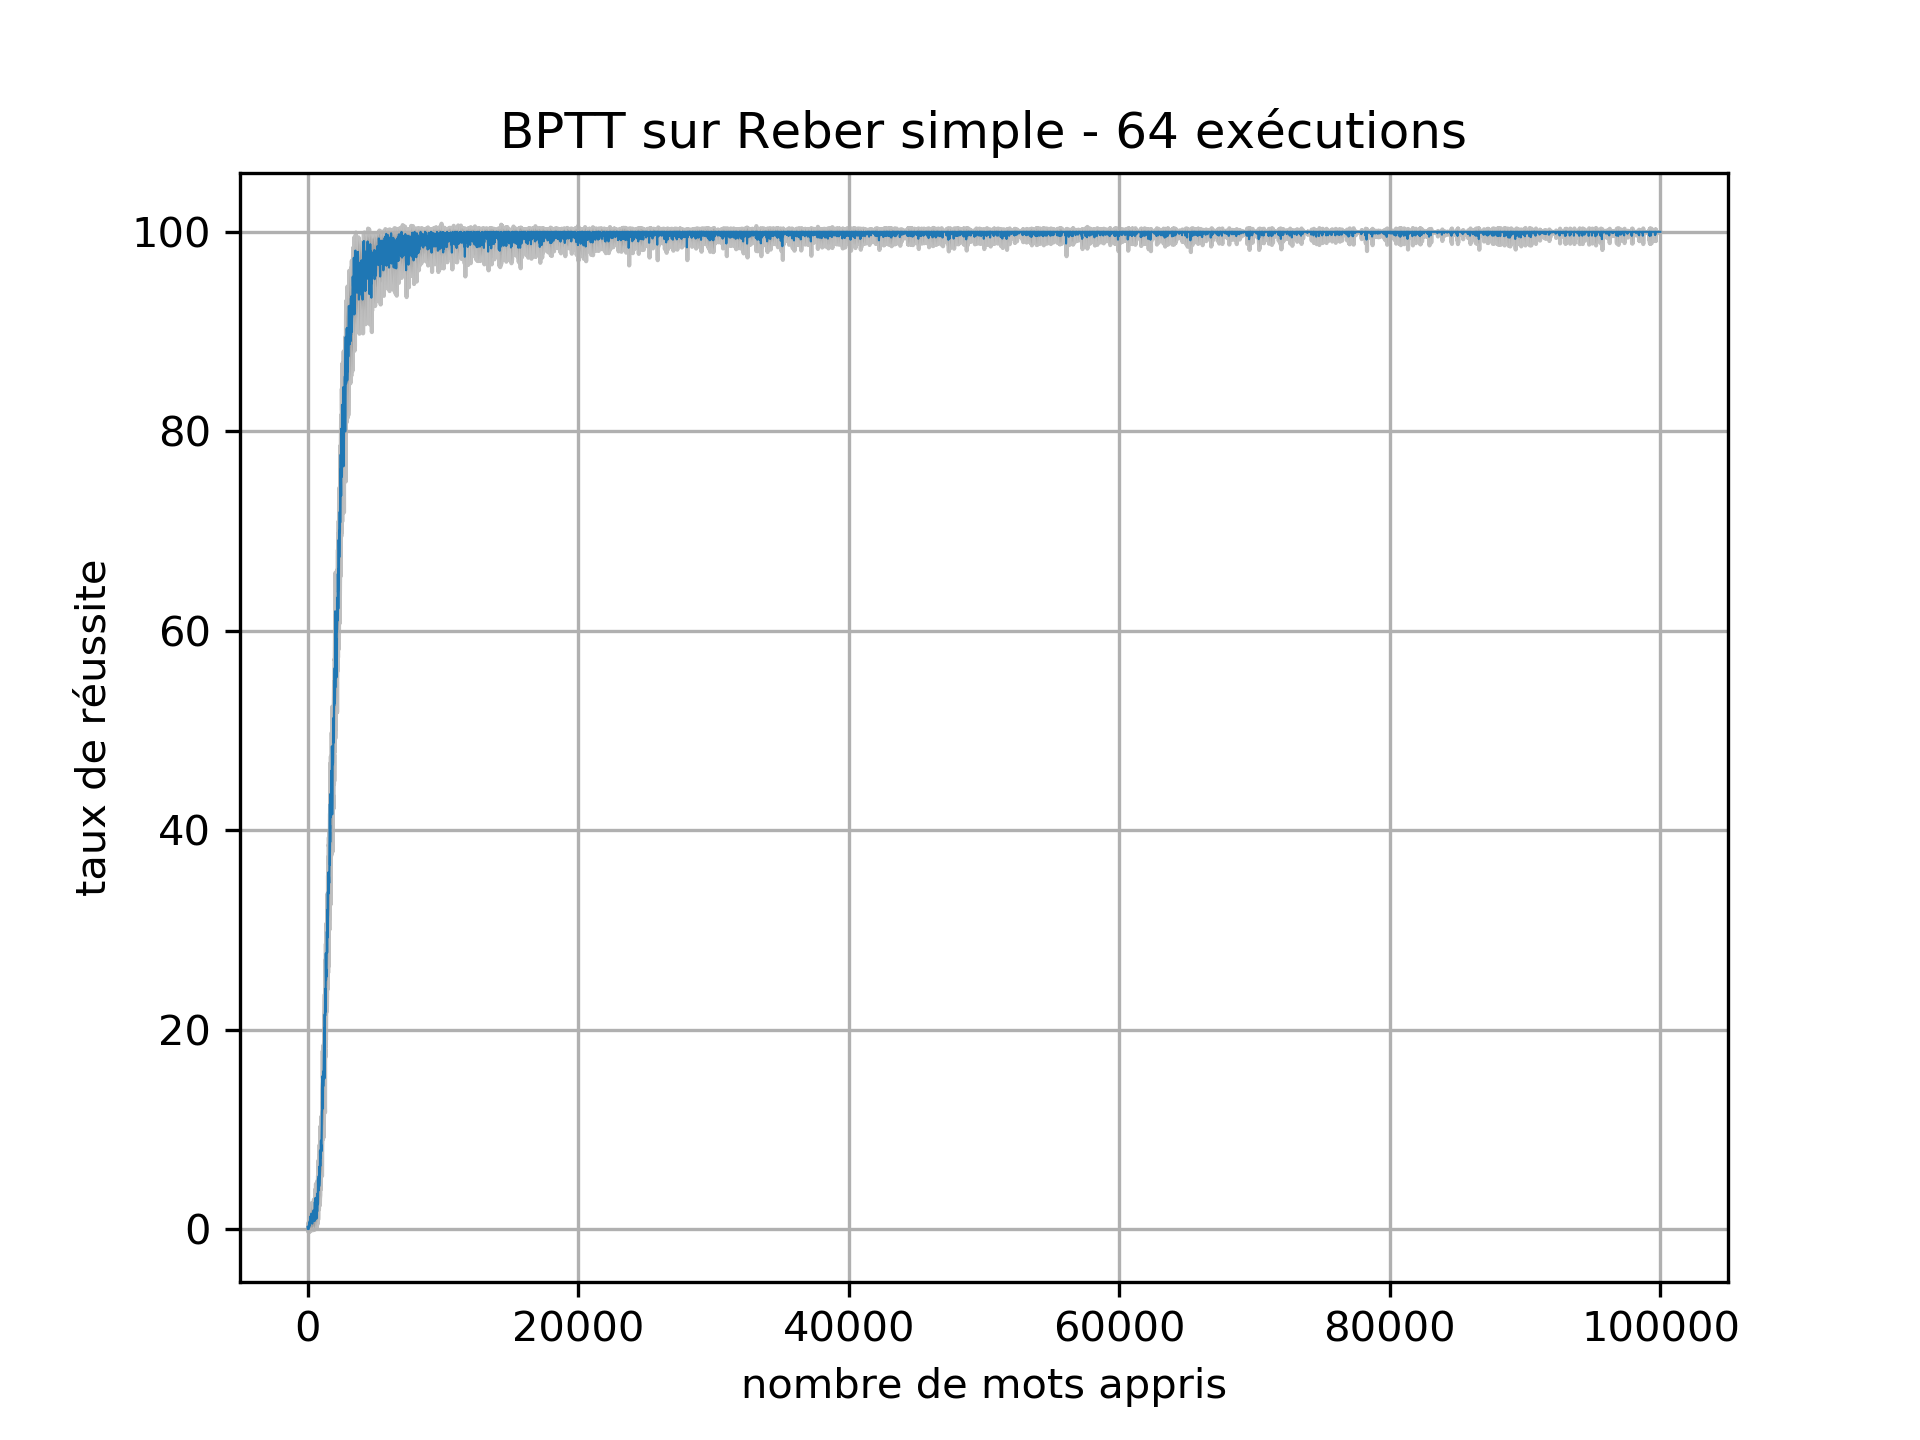
\includegraphics[width=0.7\textwidth]{images/results/bptt_simplereber_ls30_lr01.png}
\caption{Apprentissage au cours du temps, BPTT sur grammaire de Reber simple}
\end{center}
\end{figure}

\medskip

On constate que le réseau apprend de manière certaine la grammaire simple : 
le taux de réussite converge très rapidement vers 100\% et l'écart type
se réduit pour ne plus valoir que 4\%.

\medskip

On peut donc conclure sur la capactité d'un réseau récurrent sur lequel on
applique l'algorithme de mise à jour des poids BPTT à apprendre et prédire les
transitions d'un gramaire de Reber simple ?

\subsection{Grammaire de Reber symétrique}
Pour une grammaire de Reber symétrique, réussite est déterminée par la prédiction
correcte de la première et la dernière transition des mots.

\medskip

Les tests ont été réalisés dans les mêmes conditions que celles de la grammaire
simple. A été évaluée la prediction du dernier carractère en fontion du premier
de la séquence. Les caractères intermédiaires n'ont pas fait l'objet de cette
expérience.

\begin{figure}[!ht]
\begin{center}
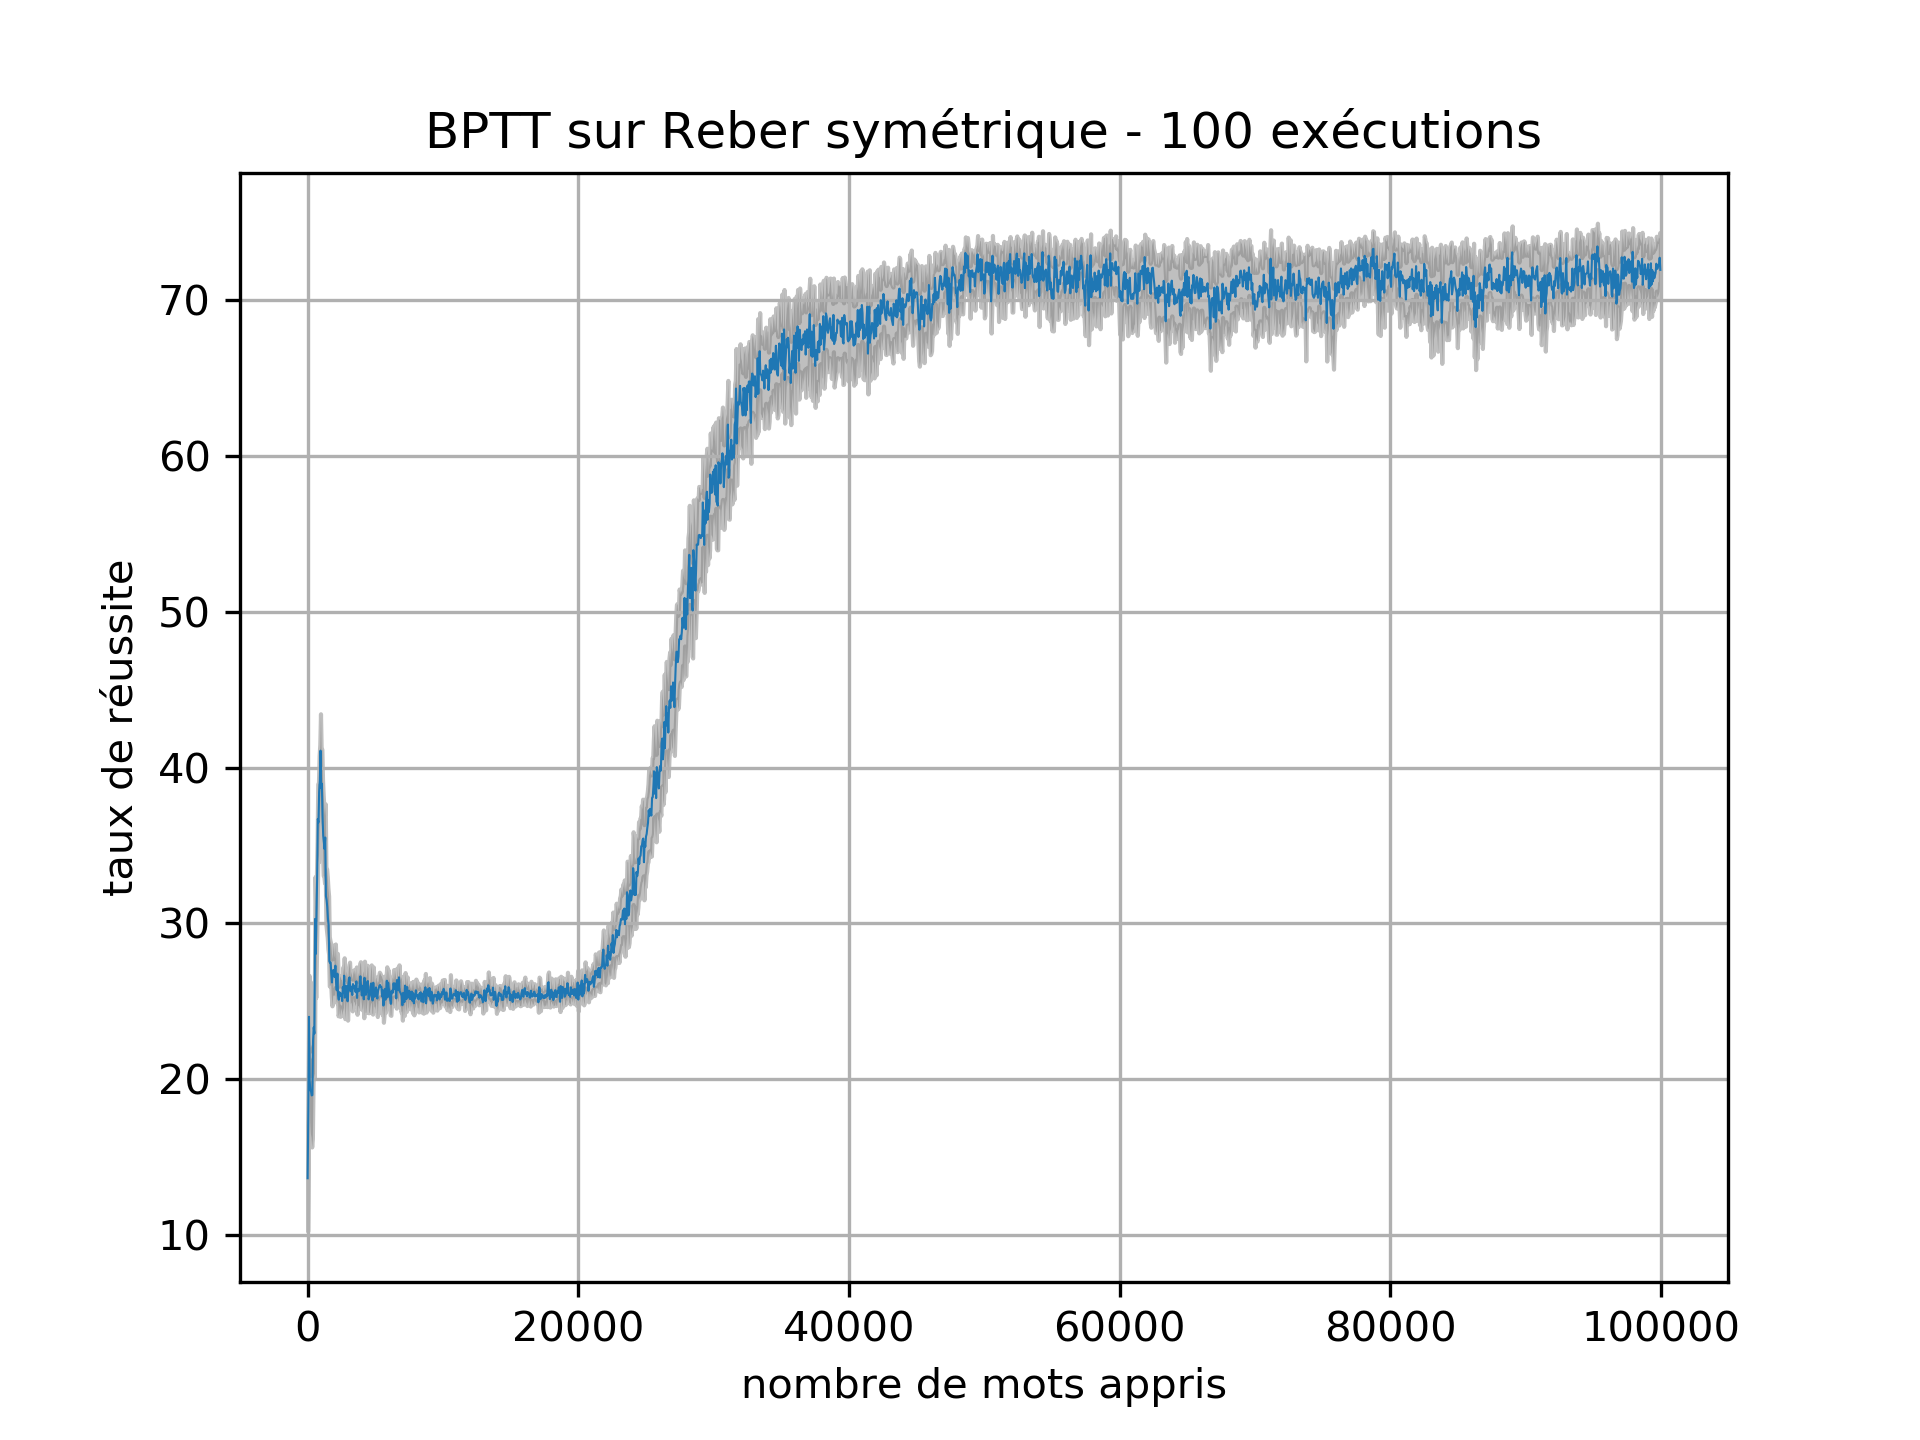
\includegraphics[width=0.7\textwidth]{images/results/bptt_doublereber_ls30_lr01.png}
\caption{Apprentissage au cours du temps, BPTT sur grammaire de Reber symétrique}
\end{center}
\end{figure}

\medskip

On constate que le réseau a plus de difficultés à prédire la dernière lettre de
la séquence. En effet, la valeur finale se situe aux alentours de 75\% de
réussite, l'éacrt type reste constant, et la convergence vers la valeur finale
s'effectue entre 20000 et 50000 mots.

% !TeX root = main.tex

\chapter{Long Short Term Memory}

Objectif principal de ce projet, l'architecture neuronale Long Short Term Memory
(LSTM) est décrite dans cette partie. Tout comme les autres architectures
neuronales, elle est constituée d'un assemblage de blocs élémentaires qui
disposent d'un ensemble de variables, appelés poids, à adapter lors de la phase
d'apprentissage afin de reproduire une fonction. Cependant, la cellule
élémentaire d'un réseau LSTM est bien plus complexe que celle d'un réseau
neuronal à perceptrons.

\medskip

La dénomination LSTM vient du fait que ce type de réseau possède une mémoire de
plus longue durée que des structures plus simples avec une seule couche de
neurones. Ainsi, il sera possible d'apprendre des fonctions telles que la
grammaire de Reber double, ou bien de générer du texte après avoir appris des
écrits de Shakespeare.

\medskip

LSTM est notamment utilisé dans des applications de reconnaissance vocale.

\medskip

\section{Théorie}
\subsection{Cellule LSTM}

La cellule LSTM est constituée de différents réseaux de perceptrons.
La principale différence avec un simple réseau à perceptrons est que la cellule
possède une mémoire. Il s'agit d'un vecteur qui sera pris en entrée (en même
temps que l'entrée au temps $t$ et la sortie du temps $t-1$, modifié par
les entrées au temps $t$ et renvoyé au temps $t+1$ dans la même cellule.

\medskip

Chaque réseau de perceptrons représente une opération sur la mémoire, tous
prennent en entrée l'entrée de la cellule au temps $t$ et sa sortie au temps
$t-1$:

\begin{itemize}
  \item La "input gate" est le réseau qui effectue des opérations d'addition
    sur la mémoire.
  \item La "block input" est le réseau qui définit les coordonnées de la mémoire
    qui seront affectées par l'input gate.
  \item La "forget gate" est le réseau qui détermine quelles coordonnées de la
    précédente mémoire garder à $t$. Ce réseau n'est pas présent dans toutes les
    implémentations, on pourra étudier l'impact de sa présence.
  \item La "output gate" est le réseau qui détermine les sorties de la cellule.
\end{itemize}

\begin{figure}[!ht]
\begin{center}
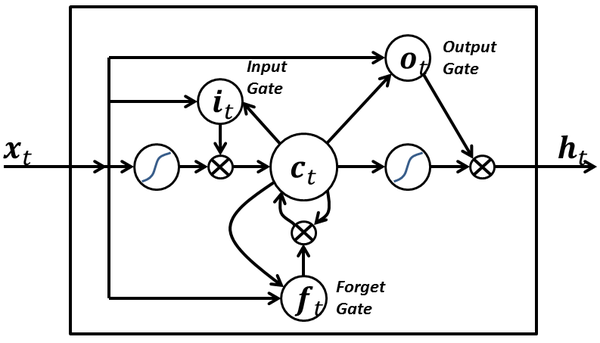
\includegraphics[width=0.6\linewidth]{images/lstm.png}
\end{center}
\caption{Cellule LSTM}
% TODO : Credits or new figure
\end{figure}

\subsection{Propagation}

Soit N la taille du vecteur de sortie et M la taille du vecteur d'entrée, on
peut définir les matrices de poids :

\begin{itemize}
  \item Poids relatifs à l'entrée : $W_z$, $W_i$, $W_f$,
    $W_o \in \mathbb{R}^{M \times N}$
  \item Poids relatifs à la sortie précédente : $R_z$, $R_i$, $R_f$,
    $R_o \in \mathbb{R}^{N \times N}$
  \item Poids des biais : $b_z$, $b_i$, $b_f$,
    $b_o \in \mathbb{R}^N$
\end{itemize}

Soit $\sigma$ la fonction d'activation sigmoide $\sigma(x)=\frac{1}{1+e^{-x}}$,
$x^t$ l'entrée au temps $t$, $y^t$ la sortie de la cellule au temps $t$, $c^t$
la mémoire de la cellule au temps $t$ et $\odot$ le produit d'Hadamard,
on peut définir les expressions suivantes pour les sorties de chaque couche de
perceptrons :

\medskip

\begin{itemize}
  \item block input :
    $$\overline{z}^t = W_z x^t + R_z y^{t-1} + b_z$$
    $$z^t = \tanh(\overline{z}^t)$$
  \item input gate :
    $$\overline{i}^t = W_i x^t + R_i y^{t-1} + b_i$$
    $$i^t = \sigma(\overline{i}^t)$$
  \item forget gate :
    $$\overline{f}^t = W_f x^t + R_f y^{t-1} + b_f$$
    $$f^t = \sigma(\overline{f}^t)$$
  \item output gate :
    $$\overline{o}^t = W_o x^t + R_o y^{t-1} + b_o$$
    $$o^t = \sigma(\overline{o}^t)$$
\end{itemize}


\subsection{Algorithmes d'apprentissage}
L'algorithme d'apprentissage est un algorithme BPTT appliqué aux cellules
LSTM considérées.

\begin{figure}[!ht]
\begin{center}
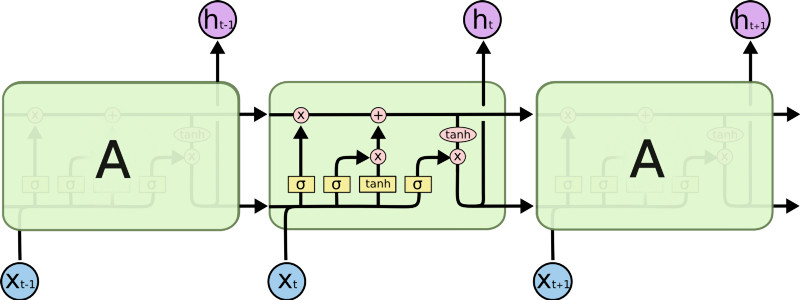
\includegraphics[width=0.8\textwidth]{images/lstm-bptt.png}
\end{center}
\caption{Dépliement du temps dans l'espace style BPTT}
% TODO : Credits or new figure
\end{figure}

\section{Implémentation}

L'implémenation est effectuée en C++ via la librairie de calcul matriciel
Eigen3. Toutes les matrices sont des objets de type Eigen::MatrixXd (matrice de
double) et les vecteurs des objets de type Eigen::VectorXd.

\medskip

L'aléatoire utilisé est celui natif en C et C++ : rand.
La génération de la graine se fait à partir du temps à la milliseconde pour
éviter une initialisation déterministe dans le cas de l'execution de plusieurs
runs consécutifs. Pour cela la librairie 'sys/time.h' est utilisée, avec un
appel propre aux systèmes UNIX.

\bigskip

\subsection{Structure de données}

Le code se décompose en plusieurs éléments :

\medskip

\begin{itemize}

  \item Les poids LSTM
  \item La cellule LSTM
  \item Le réseau LSTM

\end{itemize}
\subsubsection{Les poids LSTM}

La classe poids regroupe toutes les matrices de poids des différents noeuds
de la cellule LSTM. Ces dernier sont : input\_gate, input\_block, output\_gate.
Pour chacun des noeuds il existe deux matrices de poids : une relative à
la sortie précédente de la cellule, et l'autre relative à l'entrée de la
cellule. Enfin, il existe aussi pour chaque noeud un vecteur de biais.

\medskip

Tous ces éléments sont amenés à être modifiés, c'est pourquoi l'on crée pour
chacun une matrice (ou un vecteur) de delta : modifications à appliquer.

\medskip

Enfin, les méthodes de l'objet poids LSTM sont le constructeur et
l'application des variations de poids (qui remet par la même occasion à 0
les delta-poids).

\subsubsection{La cellule LSTM}

La cellule LSTM est l'objet élémentaire du réseau. Elle est créée en prenant
pour arguments un pointeur vers un objet de type poids, et les informations de
dimentions d'entrée et sortie.

\medskip

Elle dispose des méthodes nécessaires à la propagation et la rétropropagation
à travers une cellule LSTM.
Pour renvoyer plusieurs vecteurs (la sortie, la mémoire) on utilise ici des
std::vector<Eigen::VectorXd> dont chaque case correspond à un vecteur que l'on
souhaite renvoyer.

\medskip

La propagation n'est rien d'autre qu'une application directe des formules de la
propagation à travers une cellule LSTM. Sont stockées certaines valeurs
intermédiaires pertinentes pour éviter leur calcul à nouveau lors de la
rétropropagation.

\medskip

Lors de la rétropropagation, les variations de poids sont calculées et ajoutées
aux attributs delta\_poids de l'objet weightsLSTM. La fonction de cout choisie
est la fonction de coût quadratique (divisée par deux), sa dérivée étant alors
la différence entre sortie obtenue et sortie attendue.

\bigskip

Les attributs sont donc les suivants :

% TODO

Les méthodes sont donc les suivantes :

% TODO

\subsubsection{Le réseau LSTM}

Le réseau LSTM est principalement constitué d'un std::vector<CellLSTM>.
A chaque temps $t_i$, une nouvelle cellule est crée et stockée à l'index i du
vector.

\medskip

La propagation s'effectue cellule par cellule, chaque cellule prenant en entrée
la sortie de la précédente à $t_{i-1}$ ainsi que l'entrée du réseau au temps
$t_i$.

\medskip

De même, la rétropropagation s'effectue de la dernière cellule du vector à
la première.

\bigskip

Les attributs sont donc les suivants :

% TODO

\bigskip

Les méthodes sont donc les suivantes :

% TODO

\section{Résultats}
Ci-dessous des représentations de l'apprentissage au cours du temps du réseau sur des
grammaires de Reber, simple et double. \\
En abscisse, le nombre de mots appris, en ordonnée le taux de réussite, testé à
intervalles réguliers sur un échantillon de données de test choisies aléatoirement
dans l'ensemble de test. \\
La zone grise correspond à l'intervalle de confiance à $95\%$ sur le nombre d'exécutions
précisé.\\
Le réseau utilisé est composé d'une couche de 30 cellules LSTM, avec un learning
rate de $0.1$.

\subsection{Grammaire de Reber simple}
Pour une grammaire de Reber simple, la réussite est déterminée par la prédiction
correcte de toutes les transitions des mots testés.

\begin{figure}[!ht]
\begin{center}
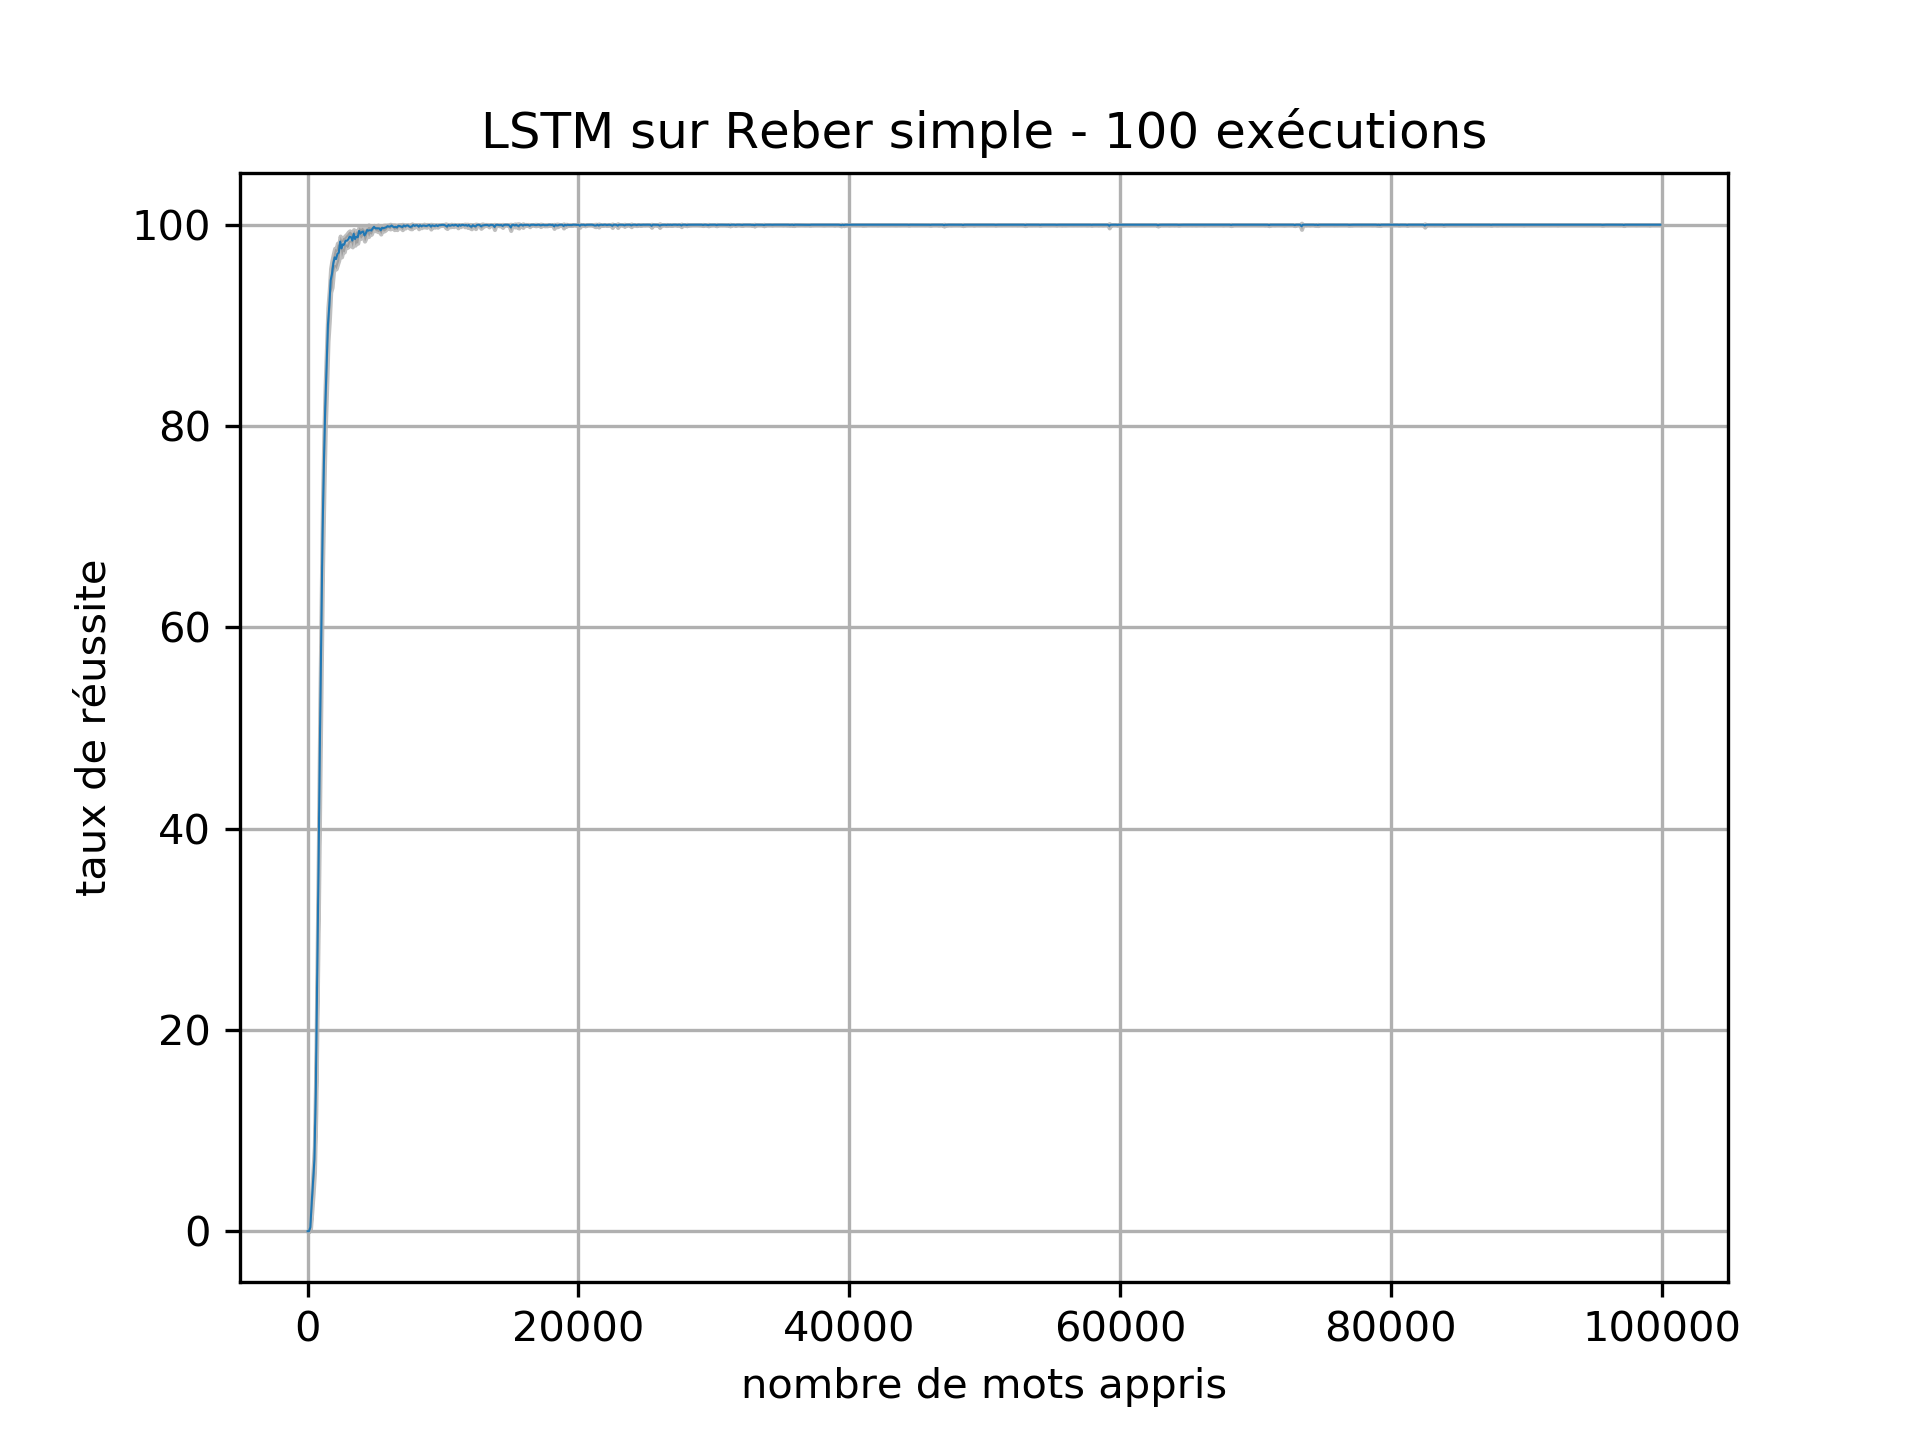
\includegraphics[width=0.8\textwidth]{images/results/lstm_simplereber_ls30_lr01.png}
\caption{Apprentissage au cours du temps, LSTM sur grammaire de Reber simple}
\end{center}
\end{figure}

\subsection{Grammaire de Reber symétrique}
Pour une grammaire de Reber symétrique, réussite est déterminée par la prédiction
correcte de la première et la dernière transition des mots testés.

\begin{figure}[!ht]
\begin{center}
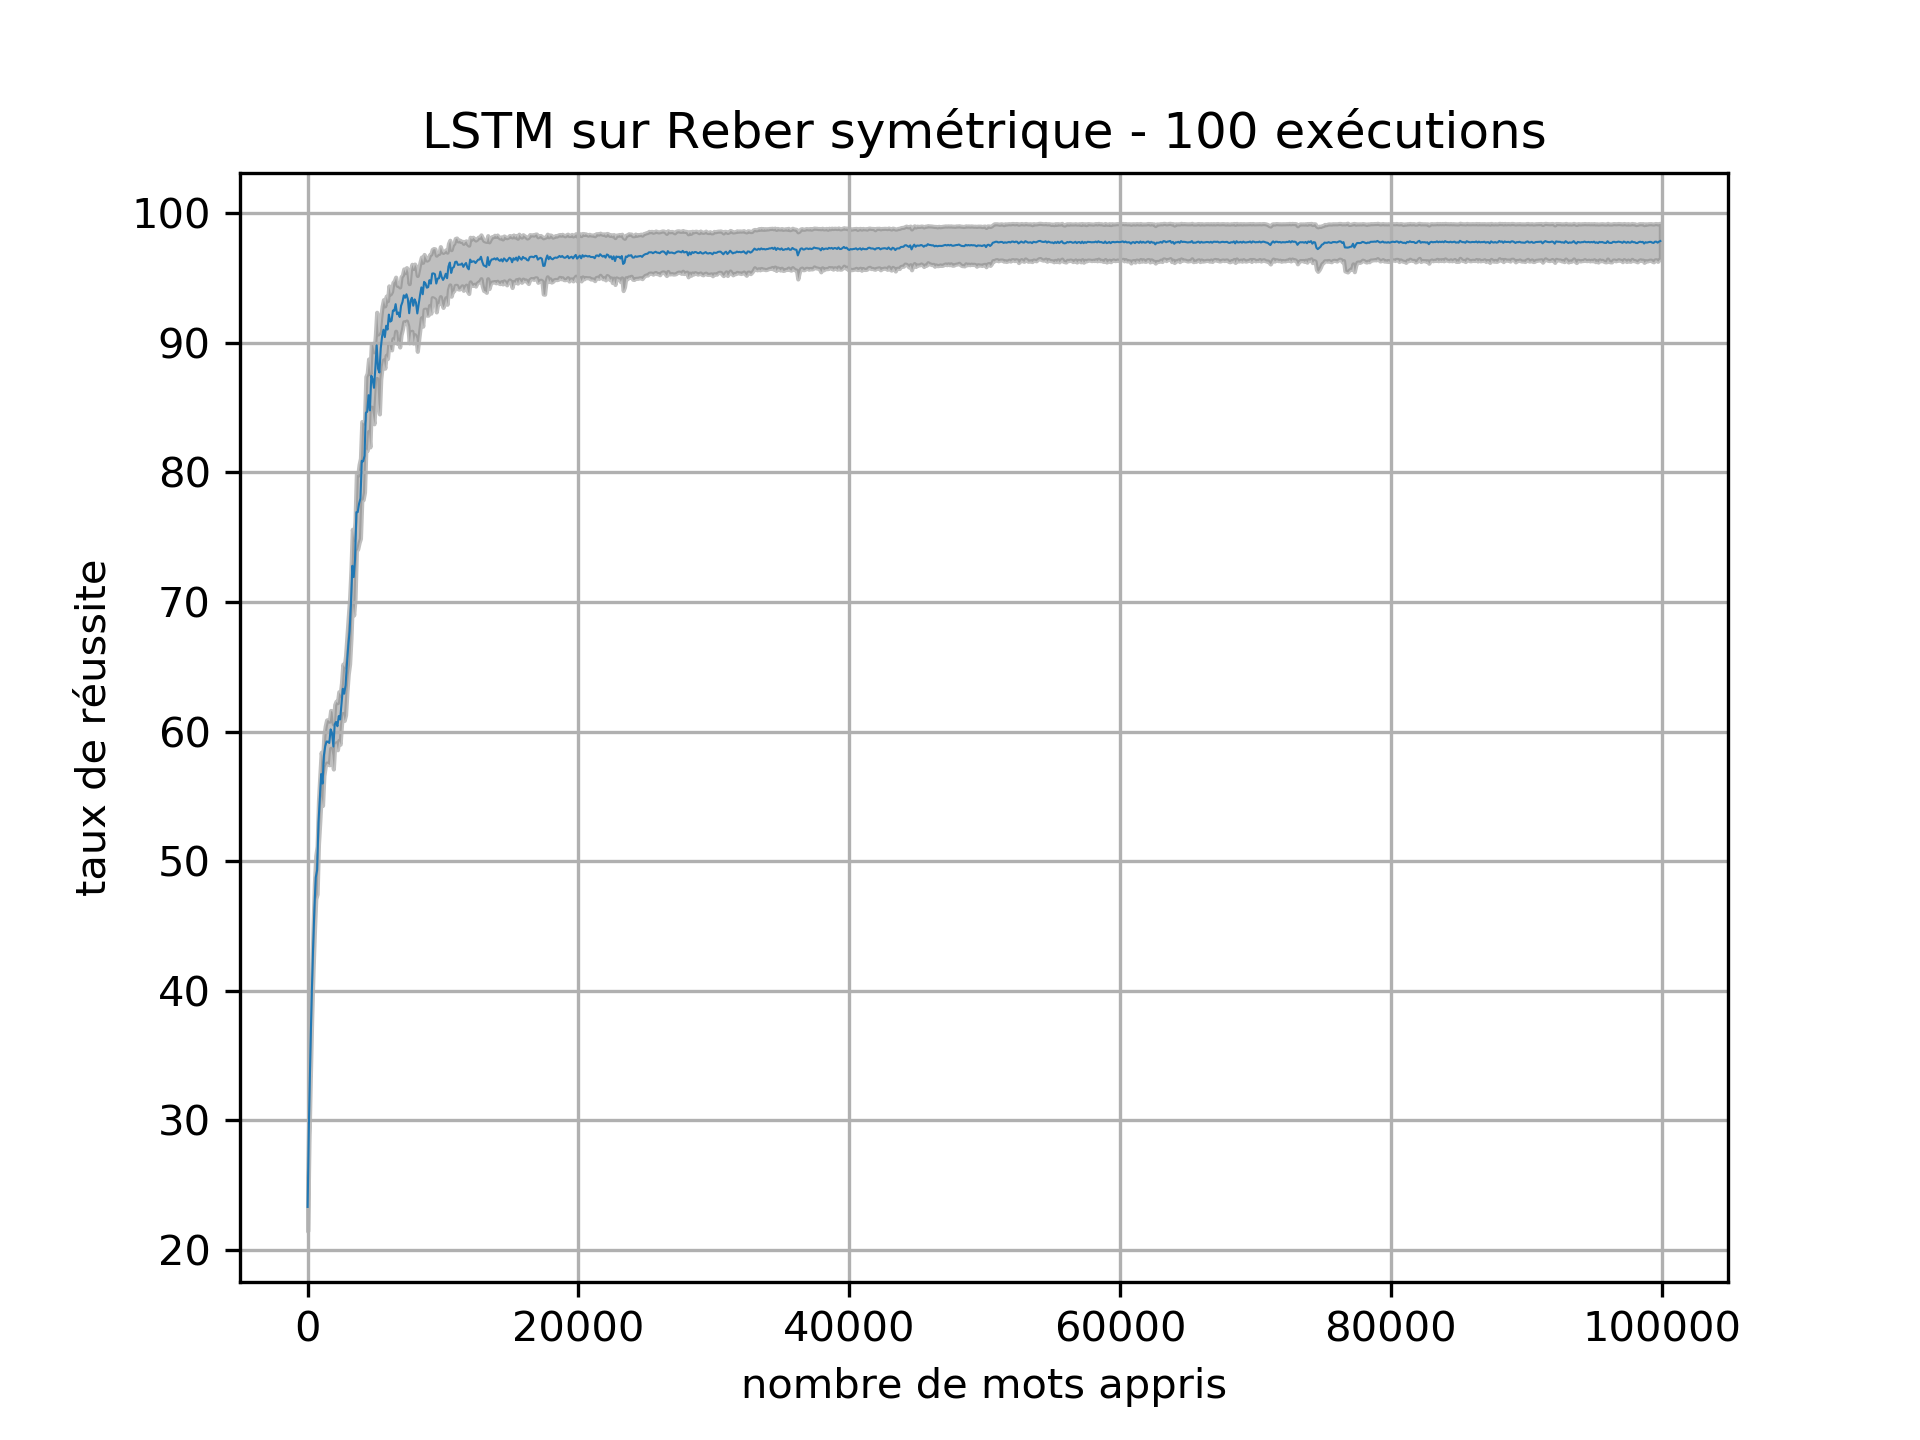
\includegraphics[width=0.8\textwidth]{images/results/lstm_doublereber_ls30_lr01.png}
\caption{Apprentissage au cours du temps, LSTM sur grammaire de Reber symétrique}
\end{center}
\end{figure}

% !TeX root = main.tex

%Ne pas numéroter cette partie
\part*{Annexes}
%Rajouter la ligne "Annexes" dans le sommaire
\addcontentsline{toc}{part}{Annexes}

%\chapter*{Annexe 1}
\addcontentsline{toc}{chapter}{Annexe 1}

%changer le format des sections, subsections pour apparaittre sans le num de chapitre
\makeatletter
\renewcommand{\thesection}{\@arabic\c@section}
\makeatother

%recommencer la numérotation des section à "1"
\setcounter{section}{0}

Intro

\section{Partie 1}

Bla

\subsection{Sous-partie 1}

Bla

\subsection{Sous-partie 2}

Bla

\subsection{Sous-partie 3}

Bla

\section{Partie 2}

Bla

\subsection{Sous-partie 1}

Bla

\subsection{Sous-partie 2}

Bla

\subsection{Sous-partie 3}

Bla
%\chapter*{Annexe 2}
\addcontentsline{toc}{chapter}{Annexe 2}

%recommencer la numérotation des section à "1"
\setcounter{section}{0}

Intro

\section*{Prérequis}
\addcontentsline{toc}{section}{Prérequis}

Bla

\begin{itemize}
\item item1;
\item item2;
\item item3;
\item item4.
\end{itemize}

Bla

\section{Partie 1}

Bla

\subsection{Sous-parie 1}

Bla

\subsection{Sous-parie 2}

Bla

\section{Partie 2}

\begin{center}
\textsc{Attention !}

\textit{Texte d'avertissement}
\end{center}

Bla

\newpage

\section{Partie 3}

Bla

\begin{figure}[!ht]
\begin{center}
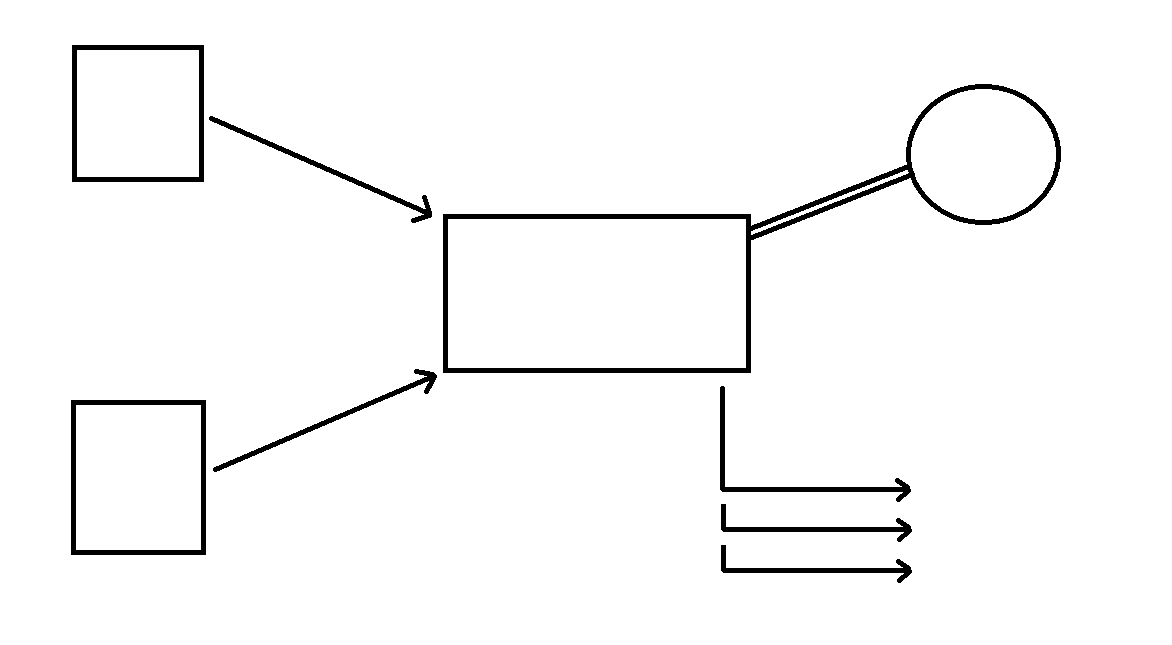
\includegraphics[height=8cm]{presentation/schema}
\end{center}
\caption[schema]{Presentation schema}
\end{figure}

\paragraph*{Paragraphe 1}
~\\
\hskip7mm

Bla

\paragraph*{Paragraphe 2}
~\\
\hskip7mm

Bla

\paragraph*{Paragraphe 3}
~\\
\hskip7mm

Bla


\newpage

%récupérer les citation avec "/footnotemark"
\nocite{*}

%choix du style de la biblio
\bibliographystyle{plain}
%inclusion de la biblio
\bibliography{pl-lstm.bib}
%voir wiki pour plus d'information sur la syntaxe des entrées d'une bibliographie

\end{document}
